
\section{Dimensional Analysis and the Buckingham Pi Theorem}
\index{Buckingham Pi Theorem}

In this section we see how dimensional analysis can be
used to discover properties of a system
without solving, or even  writing down,
any differential equations.

Every measured quantity involves units of measurement.
The units provide a standard for the dimension being measured.
For example, a ruler can be 12 inches long.  The inch is a unit used
to measure the dimension of length.  Similarly, one second is a
unit which measures the dimension of time.  There are many other
units to measure the dimensions length and time.  We can
scale the units to be any other units along that dimension but we cannot use
units from one dimension to measure quantities in a different dimension.

The fundamental observation that all equations 
relating measurable quantities have the same dimensions on both sides 
allows us to derive some relationships without knowing very much about 
the system at all.

\subsection{Dimensional Homogeneity.}
We begin with the notion of \emph{dimensional
homogeneity}.
The statement that you can't equate apples with oranges is a statement 
about the dimensional homogeneity of all equations describing the world.
Stated precisely,
an equation is \emph{dimensionally homogeneous}
if it is true regardless of the system
of units that is used to measure the parameters
or variable in the equation.

Alternatively we could state that dimensionally homogeneous equations 
can be made dimensionless (neither side requires any units) through division.
Indentifying dimensionless (also called  nondimensional) equations 
and dimensionless parameters for a given problem often provides 
information about relationships between the relevant measureable quantities.
\begin{xexample}
Consider the equation
\begin{equation}
   s = \frac{gt^2}{2}
\label{eqn:freefall}
\end{equation}
This is the equation for the
distance $s$ that an object will fall when released
at $t=0$ in a constant gravitational field.
If we use units of feet for distance and seconds
for time, then $g=32$ ft/sec$^2$.
Suppose we convert to the units miles and hours
for distance and time, respectively.
We use a bar to indicate variables in the 
new units.  We have $s = 5280\bar{s}$ (there
are 5280 feet per mile), and $t = 3600\bar{t}$
($3600$ seconds per hour).
Finally we express $g$ in the new units:
since $1 \,\textrm{ft} = (1/5280) \,\textrm{miles}$, and
$1 \,\textrm{sec} = (1/3600) \,\textrm{hr}$, we have
$g = 32$ ft/sec$^2$ becomes $\bar{g} = 32 (3600^2/5280)$
miles/hr$^2$.
Let's substitute the new variables into
\eqref{eqn:freefall}:
\begin{equation}
\begin{split}
   5280\bar{s} & = \frac{g\left(3600\bar{t}\right)^2}{2} \\
   \bar{s} & = \frac{3600^2}{5280} \frac{g\bar{t}^2}{2} \\
   \bar{s} & = \frac{\bar{g}\bar{t}^2}{2}
\end{split}
\end{equation}
The new equation involving $\bar{s}$, $\bar{t}$ and $\bar{g}$
is the same as the original equation.
This is an example of a dimensionally homogeneous equation.

The equation can be written in nonodimensional form as 
\begin{equation}
  2= \frac{gt^2}{s} \mbox{ or } 1= \frac{gt^2}{2s}.
\end{equation}
The dimensions of $g$, $s$ and $t$ ensure that any equation involving only these 
3 quantities will show that $s$ is proportional to $g$ and proportional to the
square of $t$.  This is the heart of the Buckingham Pi theorem.
\end{xexample}

\medskip
The power of dimensional analysis is based on the
fundamental observation that
\emph{equations that arise from physical laws
or real-world problems are dimensionally homogeneous}.
The number of parameters in such an equation can generally
be reduced, and this can lead to a better understanding
of the system being studied.

\subsection{The Period of a Pendulum.}
We consider a frictionless pendulum, as shown in
Figure~\ref{fig:pendulum}.
\begin{figure}
\centerline{\includegraphics[width=2in]{fig/pendulum.eps}}
\caption{A pendulum of length $l$, mass $m$, acted on
by gravity, released from the initial angle
$\theta_0$ with zero velocity.}
\label{fig:pendulum}
\end{figure}
Table~\ref{tbl:pendulumparams} lists the parameters
and their dimensions.
(Note that angles, when expressed in radians,
are actually dimensionless since they are the ratio of two lengths:
the length traveled around a circle and that circle's radius.  
Degrees are also dimensionless ``units" for angles as they are the ratio
of the distance traveled around a circle to the distance around the whole 
circle times a scaling factor of 360 to simplify arithmetic.)
\begin{table}
\centerline{%
\begin{tabular}{|c|l|l|}
  \hline
  Parameter & Meaning & Dimension \T \B \\
  \hline
    $l$  & length of the pendulum  & $\mathcal{L}$ \T \B \\
    $m$  & mass of the pendulum bob & $\mathcal{M}$ \\
    $g$  & gravitational acceleration & $\mathcal{LT}^{-2}$ \T \B \\
    $\theta_0$ &  initial angle & $1$ \\
    $T$ & period of the oscillation & $\mathcal{T}$ \\
  \hline
\end{tabular}
\vspace{0.25cm}
}
\caption{The list of variables and parameters for the pendulum,
along with their dimensions.
$\mathcal{L}$ means \emph{length},
$\mathcal{M}$ means \emph{mass}, and
$\mathcal{T}$ means \emph{time}.
The initial angle $\theta_0$ is dimensionless.}
\label{tbl:pendulumparams}
\end{table}
We consider an experiment in which we displace the pendulum
by an angle $\theta_0$, and release it with no initial
velocity.
Since we are ignoring friction, we expect the pendulum
to oscillate.  This oscillation will have some period
$T$. (The period is the time required to complete one
oscillation.)
We would like to know how the period depends on
the other parameters in the problem.
First, we'll try to determine if all these parameters
are really \emph{independent}.
To do this, we'll try to find all the
nontrivial different ways that they can be
combined to form dimensionless products.
Our goal is to find the \emph{dimensionless
parameters}.

Consider the product
\begin{equation}
   \pi = T^a l^b m^c g^d \theta_0^e
\end{equation}
We want to choose $a$, $b$, $c$, $d$ and $e$ so that
the new parameter $\pi$ is dimensionless.
(Note: $\pi$ is the name of a parameter.
We are not using $\pi = 3.1415\ldots$.)
The dimensions of $\pi$ are
\begin{equation}
  \mathcal{T}^a \mathcal{L}^b \mathcal{M}^c
     \left(\mathcal{LT}^{-2}\right)^d
     = \mathcal{T}^{a-2d}\mathcal{L}^{b+d}\mathcal{M}^c.
\end{equation}
We want $\pi$ to be dimensionless, so we want
\begin{equation}
\begin{split}
  a-2d & = 0 \\
  {b+d} & = 0 \\
  c  & = 0
\end{split}
\end{equation}
This is a linear equation for the unknown $a$, $b$, $c$, and
$d$. Actually, $e$ is also an unknown, but it only shows
up in the exponent of $\theta_0$, and $\theta_0$ is 
already dimensionless, so we know $e$ is arbitrary.
It is not difficult to solve the above system of
equations, but I will still rewrite it in matrix form, and
I'll include $e$ in the system:
\begin{equation}
   \begin{bmatrix}
       1 & 0 & 0 & -2 & 0 \\
       0 & 1 & 0 & 1  & 0 \\
       0 & 0 & 1 & 0  & 0 \\
       0 & 0 & 0 & 0 & 0  \\
   \end{bmatrix}
   \begin{bmatrix}
       a \\ b \\ c \\ d \\ e
   \end{bmatrix}
   =
   \begin{bmatrix}
       0 \\ 0 \\ 0 \\ 0
   \end{bmatrix}
   \label{eqn:linear_sys_for_nondim_params}
\end{equation}
which we can write more concisely as
\begin{equation}
   A \BP = \mathbf{0}
\end{equation}
where $A$ is the \emph{dimension matrix}
and  $\BP$ is the vector of the powers
$a$, $b$, $c$, $d$, $e$.
Each nontrivial solution to the
linear algebra problem provides a way
to combine the dimensional parameters
into a nondimensional product.
Note, however, that if
$\BP = \left[a,b,c,d,e\right]^{\textsf{T}}$ is a solution,
then so is $r\left[a,b,c,d,e\right]^{\textsf{T}} = \left[ra,rb,rc,rd,re\right]^{\textsf{T}}$
for any constant $r$.
Since
\begin{equation}
  T^{ra}l^{rb} m^{rc} g^{rd} \theta_0^{re}
   = \left(T^a l^b m^c g^d \theta_0^e\right)^r ,
\end{equation}
multiples of a solution to \eqref{eqn:linear_sys_for_nondim_params}
do not really identify new combinations of
parameters.
Thus, all we need is a set of
\emph{linearly independent} solutions
to \eqref{eqn:linear_sys_for_nondim_params}.
(To use the lingo from linear algebra, we need
a \emph{basis for the null-space of $A$}.)
In this case, we see that the system~\eqref{eqn:linear_sys_for_nondim_params}
is already in reduced row echelon form, and
the solution can be written
\begin{equation}
  \BP = c_1\begin{bmatrix} 2 \\ -1 \\ 0 \\ 1 \\ 0 \end{bmatrix} +
      c_2 \begin{bmatrix} 0 \\ 0 \\ 0 \\ 0 \\ 1 \end{bmatrix} 
\end{equation}
where $c_1$ and $c_2$ are arbitrary.  Thus a basis for the
null-space of $A$ is
given by the two vectors in the above solution.
So one nondimensional parameter is
\begin{equation}
   \pi_1 = T^2 l^{-1} m^0 g^1 \theta_0^0
         = \frac{gT^2}{l}
\end{equation}
and another (which we already knew) is
\begin{equation}
   \pi_2 = T^0 l^0 m^0 g^0 \theta_0^1
         = \theta_0 .
\end{equation}


Presumably there \emph{is} some relationship
among $l$, $m$, $g$, $\theta_0$, and the
period $T$. We don't know what it is, so we'll
just assume it can be written in the form
\begin{equation}
   f(T,l,m,g,\theta_0) = 0,
   \label{eqn:assume}
\end{equation}
where $f$ is dimensionally homogeneous.
The fundamental result that we will now use
is known as the \emph{Buckingham Pi Theorem}.\index{Buckingham Pi Theorem}
It says that a dimensionally homogeneous
relation is equivalent to another relation
expressed  in terms of only the independent
nondimensional parameters $\pi_i$.
For our example, the Buckingham Pi Theorem
implies that there is a function $F$
for which
\begin{equation}
   F(\pi_1,\pi_2) = 0.
   \label{eqn:bpthmresult}
\end{equation}
Thus it must be possible to
express the relation assumed in
\eqref{eqn:assume} in the simpler form
\begin{equation}
    F\left(\frac{gT^2}{l},\theta_0\right) = 0.
\end{equation}
Equation \eqref{eqn:bpthmresult}
is an implicit relation between $\pi_1$ and $\pi_2$.
We expect that for most values of $\pi_1$ and
$\pi_2$, we can solve for $\pi_1$ in terms
of $\pi_2$.  That is, we can write
\eqref{eqn:bpthmresult} as
\begin{equation}
    \pi_1 = h(\pi_2)
    \label{eqn:bpthmsolved}
\end{equation}
where $h$ is some function.
(In principle, the function $h$ exists,
but the dimensional analysis performed here
tells us nothing about the nature of $h$.)
Substituting the formulas for $\pi_1$ and $\pi_2$
into \eqref{eqn:bpthmsolved} gives
\begin{equation}
    \frac{gT^2}{l} = h(\theta_0),
\end{equation}
or
\begin{equation}
    T = \sqrt{\frac{l}{g} h(\theta_0)}
      = \sqrt{\frac{l}{g}}\, \hat{h}(\theta_0)
\end{equation}
where $\hat{h}(\theta_0) = \sqrt{h(\theta_0)}$.
With this result, we can predict how the period
of the oscillation of the pendulum depends on
the parameters $g$ and $l$, without actually
solving (or even writing down) the differential
equations that describe the motion.

For example, suppose a pendulum of length $l_1$ has
period $T_1$ when released from angle $\theta_0$.
If the length is doubled and the pendulum
is released from the same angle, the new period
must be
\begin{equation}
   T_2 = \sqrt{\frac{l_2}{g}} \, \hat{h}(\theta_0)
       = \sqrt{\frac{2l_1}{g}} \, \hat{h}(\theta_0)
       = \sqrt{2}\sqrt{\frac{l_1}{g}} \, \hat{h}(\theta_0)
       = \sqrt{2} \, T_1.
\end{equation}
Thus, doubling the length should cause the period
to increase by a factor of $\sqrt{2}$.

We can also compare the behavior of a pendulum
on Earth to its behavior on Mars.
The gravitational constant
$g_M$ on Mars is roughly one-third that of Earth's
gravitational consant $g_E$.
If, for a given initial angle $\theta_0$ and length $l$,
the period of the oscillation on Earth is $4$ seconds,
then on Mars the period will be
\begin{equation}
\begin{split}
    T_M = \sqrt{\frac{l}{g_M}} \, \hat{h}(\theta_0)
        = \sqrt{\frac{l}{g_E/3}} \, \hat{h}(\theta_0)
	= \sqrt{3}\, \sqrt{\frac{l}{g_E}} \, \hat{h}(\theta_0)
	= \sqrt{3}\, T_E
	& = \sqrt{3}\, 4 \\
	& \approx 6.9 \; \textrm{seconds.}
\end{split}
\end{equation}

\subsection{Another Example: Periodic Drug Doses}
We consider the concentration of a drug
in the bloodstream of an individual when the drug is administered
periodically.  We'll look at a simple model that involves
both a differential equation and a discrete map.  We'll also
see another example of using dimensional analysis.

\subsection*{Clearing of a Drug from the Bloodstream}
There is a variety of mechanisms for a drug to be cleared from the
bloodstream. Organs in the body may actively absorb the drug, the drug
may react with other chemicals in the bloodstream,
or the drug may naturally breakdown
into simpler components.
The simplest model of how a drug is cleared from the bloodstream
results from assuming that the rate of loss of the drug is
proportional to the concentration of the drug. If $c(t)$ is the
concentration of the drug at time $t$, the differential equation
for this simple model is
\begin{equation}
  \frac{dc}{dt} = -r c,
\label{eqn:decay}
\end{equation}
where $r>0$ is the proportionality constant that determines
the rate of clearance.
We know that the solution to this equation
is $c(t) = c_0 e^{-rt}$, where $c_0$ is the concentration
at time $t=0$.

Equation~\eqref{eqn:decay}
is the same as the equation for the decay of
radioactive materials, so we can define the
\emph{half-life} of the drug. This is the time
required for the amount of the drug to be reduced
to half the original amount.
For example, according to an article on
\textbf{Slate} by Sam Schechner\footnote{\texttt{http://slate.msn.com/id/2110979/}, Dec. 13, 2004}
about the poisoning of Ukrainian president
Viktor Yushchenko, some isomers of 
dioxin have a half-life of more than seven years.
If a drug has a half-life of seven years, then
\begin{equation}
   c(7) = c_0e^{-7r} = \frac{c_0}{2},
\end{equation}
which implies
\begin{equation}
   r = \frac{\ln 2}{7} \approx 0.0990,
\end{equation}
where we assume $t$ is measured in years, so that 
$r$ has the units of years$^{-1}$.
\begin{question}
Suppose a drug has a half-life of seven years.
(a) How long will it take for the amount of the drug to
be reduced to one-quarter of the original amount?
(b) How long will it take to be reduced to one percent of the 
original amount?

\hfill \textbf{Answers:} (a) 14 years, (b) 46.5 years.
\end{question}

\subsection*{Administering a Drug with Periodic Doses}
We now suppose that a drug is administered periodically.
That is, every $h$ time units, a dose is administered that
increases the concentration by $b$.
(If the \emph{amount} administered is $a$, and the volume
of the blood in bloodstream is $V$, then $b=a/V$.
We will work with $b$ from here on.)
We assume that the dose causes an instantaneous increase
in the concentration.  This is probably a
good assumption for a drug administered by an injection.
Whether this is a good assumption for a drug taken
orally depends on the properties of the drug.
Alcohol, for example, enters the bloodstream fairly
rapidly, so the instantaneous increase in concentration
is probably a reasonable approximation for alcohol.

We assume that the first dose is administered at time $t=0$, and
the concentration of the drug in the bloodstream before then
is zero.  At $t=0$ the concentration jumps to $b$, and then
for $0 < t < h$, the concentration decays according
to~\eqref{eqn:decay}.  At $t=h$, another dose is administered,
and the concentration increases by $b$. The concentration then decays
for $h < t < 2h$, and the process continues.
We expect the plot of the concentration to look like
the graph shown in Figure~\ref{fig:PeriodicDrugDosePlot}.
\begin{figure}
\centerline{%
\includegraphics[angle=270,width=4in]{python_PeriodicDrugDose/PeriodicDrugDosePlot.eps}
}
\caption{A plot of the concentration $c(t)$ for a drug administered
periodically.  In this example, $r=0.3$, $h=2$ and $b=1$.
At $t=0, h, 2h, \ldots$, $c(t)$ increases by $b$; otherwise
the concentration decays according to~\eqref{eqn:decay}.}
\label{fig:PeriodicDrugDosePlot}
\end{figure}


Let $x_n$ be the concentration at the moment before
a new dose is administered.
It is clear the graph of $c(t)$ consists of
regions of exponential decay, separated by jumps.  What we would like to
know is what happens to $x_n$ as $n$ increases?
Does $x_n$ increase without bound? Or does $x_n$ approach
some value asymptotically?  If so, what value does is approach?

\subsection*{Dimensional Analysis of $\pmb{x_{\infty}}$}
We'll find the exact formula for $x_n$ in the next section.
In this section, we
assume that $x_n$ approaches a finite value $x_{\infty}$
asymptotically as $n\rightarrow\infty$.
We use dimensional analysis to determine
(as far as possible) how $x_{\infty}$
depends on the other parameters.

We use the procedure that we saw for the period of the pendulum
in an earlier lecture.  Our first task is to find all
the \emph{independent} nondimensional parameters.
We list all the relevant parameters along with their
dimensions in Table~\ref{tbl:params}.
\begin{table}
\centerline{%
\begin{tabular}{|c|l|l|}
  \hline
  Parameter & Meaning & Dimension \T \B \\
  \hline
    $r$  & proportionality constant for the clearance of the drug  & $\mathcal{T}^{-1}$ \T \B \\
    $h$  & time period  & $\mathcal{T}$ \\
    $b$  & instantaneous change in concentration due to each dose & $\mathcal{C}$ \T \B \\
    $x_{\infty}$ &  asymptotic concentration just before the next dose  & $\mathcal{C}$ \\
  \hline
\end{tabular}
\newline
\vspace{0.2cm}
}
\caption{The list of variables and parameters along with their dimensions.
$\mathcal{T}$ means \emph{time} and $\mathcal{C}$ means a
\emph{concentration}.
(In a problem with a wider variety of parameters, we might want to
express concentration as an \emph{amount} $\mathcal{A}$ divided by
a \emph{volume} $\mathcal{V}$ or even divided by the cube of a
\emph{length} $\mathcal{L}$, but this is not necessary in this
case.)}
\label{tbl:params}
\end{table}
We see that $\pi_1=rh$
and $\pi_2=x_{\infty}/b$
are nondimensional combinations of the parameters.
With a little thought, we could probably
convince ourselves that these are the \emph{only} nontrivial
(or independent) combinations.
(For example, $rhb^2/x_{\infty}^2$ is nondimensional,
but it is equivalent to
$\pi_1/\pi_2^2$, so it is not really a ``new'' parameter.)
However, for the sake of
pedagogy, we will follow the formal procedure, and pretend
we didn't see the ``obvious'' choices.

We must choose exponents $\alpha$, $\beta$, $\gamma$ and $\delta$
such that
\begin{equation}
   \pi = r^{\alpha} b^{\beta} h^{\gamma} x_{\infty}^{\delta}
\label{eqn:nondimparam}
\end{equation}
is dimensionless.  Substituting in the dimensions from 
Table~\ref{tbl:params}, we require
\begin{equation}
   \left(\mathcal{T}^{-1}\right)^{\alpha} \mathcal{C}^{\beta}
       \mathcal{T}^{\gamma} \mathcal{C}^{\delta} = \mathcal{T}^0\mathcal{C}^0 = 1
       \quad\implies\quad
       \mathcal{T}^{-\alpha+\gamma}\mathcal{C}^{\beta+\delta}
        = \mathcal{T}^{0}\mathcal{C}^{0}.
\end{equation}
This results in the linear system of equations
\begin{equation}
\begin{split}
   -\alpha + \gamma & = 0, \\
    \beta + \delta & = 0. \\
\label{eqn:pdd:linearsys}
\end{split}
\end{equation}
This is easy enough to solve: $\alpha = \gamma$ and $\beta = -\delta$,
where $\gamma$ and $\delta$ are arbitrary. 
%Equivalently, we can express this as
%\begin{equation}
%  \alpha = p, \quad \beta = -q, \quad \gamma = p, \quad \delta = q,
%\end{equation}
%where $p$ and $q$ are arbitrary parameters.
%In vector form,
%\begin{equation}
%\begin{bmatrix} \alpha \\ \beta \\ \gamma \\ \delta \end{bmatrix}
%  =
%\begin{bmatrix} p \\ -q \\ p \\ q \end{bmatrix}
%  =
%p\begin{bmatrix} 1 \\ 0 \\ 1 \\ 0 \end{bmatrix} +
%q\begin{bmatrix} 0 \\ -1 \\ 0 \\ 1 \end{bmatrix} .
%\end{equation}
%A \emph{basis} for the solution set of~\eqref{eqn:pdd:linearsys}
%is given by the vectors $\left\{[1,0,1,0],[0,-1,0,1]\right\}$ (written as
%row vectors for convenience).
%Each basis vector gives us exponents that we can plug into~\eqref{eqn:nondimparam} to form a nondimensional parameter.
Thus we have found (as expected) that there are only two
independent nondimensional parameters:
\begin{equation}
  \pi_1 = r^1 b^0 h^1 x_{\infty}^0 = rh, \quad \textrm{and}\quad
  \pi_2 = r^0 b^{-1} h^0 x_{\infty}^1 = \frac{x_{\infty}}{b}. 
\end{equation}

Now we assume that there is some functional relationship
among $r$, $h$, $b$ and $x_{\infty}$.  Since we don't know
what it is, we'll assume the general form
\begin{equation}
  f(r,h,b,x_{\infty}) = 0.
\end{equation}
We expect $f$ to be dimensionally homogeneous; then the
Buckingham Pi Theorem\index{Buckingham Pi Theorem} implies that there is an equivalent
relationship of the form
\begin{equation}
   F(\pi_1, \pi_2) = 0.
\label{eqn:F}
\end{equation}
Moreover, we expect that for most values of $\pi_1$
and $\pi_2$, this equation can be solved for $\pi_2$
in terms of $\pi_1$. That is, there is some function
$G$ such that~\eqref{eqn:F} is equivalent to
\begin{equation}
   \pi_2 = G(\pi_1).
\end{equation}
Substituting in the definitions of $\pi_1$ and $\pi_2$ gives
\begin{equation}
   \frac{x_{\infty}}{b} = G(rh),
\end{equation}
or
\begin{equation}
   x_{\infty} = bG(rh).
\end{equation}
This gives us the form of the equation that will result if
we can solve for $x_{\infty}$ in terms of $r$, $h$ and $b$.
That is, $x_{\infty}$ \emph{must} be
a product of $b$ and some function of $rh$ only.

%This problem is actually simple enough that we can
%solve for $x_{\infty}$ exactly.
%In the steady-state behavior of $c(t)$, the decrease
%in the concentration during the time interval
%between doses must be exactly $b$.
%For convenience, let us shift our time axis
%so that the concentration has just jumped to 
%$c_{\textrm{max}}$ at $t=0$.
%Then $c(h) = c_{\textrm{max}}e^{-rh}$, and the change in the
%concentration is
%\begin{equation}
%   c(0)-c(h) = c_{\textrm{max}}-c_{\textrm{max}}e^{-rh} = c_{\textrm{max}}(1-e^{-rh}).
%\end{equation}
%This must equal $b$:
%\begin{equation}
%   c_{\textrm{max}}(1-e^{-rh})=b \implies
%        c_{\textrm{max}} = \frac{b}{1-e^{-rh}} 
%\end{equation}
%Finally, since $x_{\infty}$ is the concentration at the
%end of the $h$ time interval (just before the next dose),
%we have
%\begin{equation}
%   x_{\infty} = c_{\textrm{max}}-b = \frac{b e^{-rh}}{1-e^{-rh}}.
%\end{equation}
%As expected, the formula has the form $bG(rh)$.
%In this case, $G(u) = \frac{e^{-u}}{1-e^{-u}}$.
%%
%\subsection*{Derivation of the Formula for $\pmb{x_{n}}$}%
%In this section,%
%\footnote{This section is not an integral part of the
%discussion of dimensional analysis.}
%we derive the actual formula for
%$x_n$. 
%You may find it helpful to label the plot in
%Figure~\ref{fig:PeriodicDrugDosePlot} using the notation
%from the following discussion.
%
%We need some additional notation to describe the
%graph shown in the figure.
%Let
%\begin{equation}
%\begin{split}
%    c(h^{-})  & = \lim_{t\rightarrow h^{-}} c(t)
%                     \quad\quad \textrm{(the limit from below),} \\
%    c(h^{+})  & = \lim_{t\rightarrow h^{+}} c(t)
%                     \quad\quad \textrm{(the limit from above).}
%\end{split}
%\end{equation}
%and define
%\begin{equation}
%   x_n = c((nh)^{-}).
%\end{equation}
%
%The instant after the first dose, we have
%\begin{equation}
%  c(0^{+}) = b.
%\end{equation}
%Then, for $0 < t < h$, we have $c(t) = be^{-rt}$, so
%\begin{equation}
%  c(h^{-}) = be^{-rh}.
%\label{eqn:x_one}
%\end{equation}
%At $t=h$, the concentration increases by $b$, so
%\begin{equation}
%  c(h^{+}) = c(h^{-})+b = be^{-rh} + b = b\left(e^{-rh}+1\right)
%\end{equation}
%Then in the next interval, the solution again decays, and we have
%\begin{equation}
%  c((2h)^{-}) = c(h^{+})e^{-rh} = b\left(e^{-rh}+1\right) e^{-rh}
%     = b\left(e^{-2rh} + e^{-rh}\right)
%\label{eqn:x_two}
%\end{equation}
%and after the jump at $t=2h$ we have
%\begin{equation}
%  c((2h)^{+}) = c((2h)^{-})+b = b\left(e^{-2rh}+e^{-rh}\right) + b
%     = b\left( e^{-2rh} + e^{-rh}+1\right)
%\end{equation}
%Once again, in the next time interval, the solution decays and we have
%\begin{equation}
%  c((3h)^{-}) = c((2h)^{+})e^{-rh} = b\left( e^{-2rh} + e^{-rh}+1\right)e^{-rh}
%    = b\left( e^{-3rh} + e^{-2rh}+e^{-rh}\right)
%\label{eqn:x_three}
%\end{equation}
%Recall that we defined $x_n = c((nh)^{-})$.
%The process that we are describing defines a one dimensional mapping
%\begin{equation}
%   x_{n+1} = (x_n+b)e^{-rh}, \quad \textrm{with $x_0=0$.}
%\end{equation}
%Equations~\eqref{eqn:x_one}, \eqref{eqn:x_two} and
%\eqref{eqn:x_three} give the formulas for the first three
%iterations of this map.
%In general, we have
%\begin{equation}
%  x_n = c((nh)^{-}) = b\left( e^{-nrh} + e^{-(n-1)rh} + \cdots + e^{-rh}\right)
%        = b \sum_{k=1}^{n} e^{-krh}
%    = b \sum_{k=1}^{n} \rho^k,
%\label{eqn:xnsum}
%\end{equation}
%where $\rho = e^{-rh}$.
%(Note that, since $r>0$ and $h>0$, we have $0 < \rho < 1$.)
%The formula in Equation~\eqref{eqn:xnsum} is a geometric sum.
%By using Equation~\eqref{eqn:geomsumfromone} from the
%appendix, we obtain
%\begin{equation}
%  x_n = b \rho\left(\frac{1-\rho^n}{1-\rho}\right)
%      = be^{-rh}\left(\frac{1-e^{-nrh}}{1-e^{-rh}}\right)
%\end{equation}
%Finally, since $\ds \lim_{n\rightarrow\infty} \rho^n = 0$, we have
%\begin{equation}
%  x_{\infty} = \frac{b\rho}{1-\rho}
%     = \frac{be^{-rh}}{1-e^{-rh}}. 
%\end{equation}
%
%The example shown earlier was for $r=0.3$, $h=2$ and $b=1$.
%With these values we find $x_{\infty} \approx 1.2164$.
%Figure~\ref{fig:PeriodicDrugDosePlotWithXinf}
%shows the result of ten periods for these parameters.
%The dashed line in this plot indicates $x_{\infty}$.
%\begin{figure}
%\centerline{%
%\includegraphics[angle=270,width=4.5in]{python_PeriodicDrugDose/PeriodicDrugDosePlotWithXinf.eps}
%}
%\caption{The graph of $c(t)$ for $r=0.3$, $h=2$, and $b=1$.
%The dashed line shows $x_{\infty} \approx 1.2164$.}
%\label{fig:PeriodicDrugDosePlotWithXinf}
%\end{figure}
%%
%
%%\newpage

\begin{exercises}
\begin{exercise}
\label{ex:Nondim_lrgmP}
Find a set of independent nondimensional parameters for the following
dimensional parameters.  The dimension of each parameter
is given in parentheses.

\centerline{$\ell$ ($\mathcal{L}$), $r$ ($\mathcal{T}^{-1}$),
$g$ ($\mathcal{LT}^{-2}$), $m$ ($\mathcal{M}$),
$P$ ($\mathcal{M}\mathcal{L}^{-1}\mathcal{T}^{-2}$)}
\end{exercise}
\end{exercises}
